\begin{abox}
	Electronics
	\end{abox}
\begin{enumerate}
	\item The circuit is as shown in figure
	\begin{figure}[H]
		\centering
		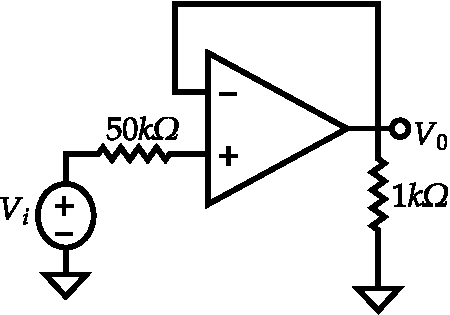
\includegraphics[height=3cm,width=4.5cm]{CE-1}
	\end{figure}
	(i) The ideal closed loop voltage gain is
	 \begin{tasks}(4)
		\task[\textbf{a.}]1
		\task[\textbf{b.}]$-1$
		\task[\textbf{c.}]$\infty$
		\task[\textbf{d.}]50 
	\end{tasks}
	\begin{answer}
		$$
		\begin{aligned}
		\text { Voltage follower circuit, } V+&=V_{i}, V-=V_{i}=V_{0}, \frac{V_{0}}{V_{i}}=1 \text {. Hence, (a) is correct answer. }\\
		\text { (ii) The open loop gain is } &A_{\text {od }}=999 \text {, then closed loop gain is }\\
		\text{(a)}\quad -0.999\qquad
		\text{(b)}\quad &0.999 \qquad
		\text{(c)}\quad 1.001 \qquad
		\text{(d)}\quad -1.001\\
		V+=V_{i}, V-=V_{0}, A_{o d}\left(V_{i}-V_{0}\right)&=V_{0}, \quad A_{o d} V_{i}=\left(A_{o d}+1\right) V_{0}, A_{o d}=999\\
		\frac{V_{0}}{V_{1}}=\frac{A_{o d}}{1+A_{o d}}&=\frac{999}{1+999}=0.99
	\end{aligned}
	$$
	So the corrext answer is \textbf{Option (b)}
	\end{answer}
	\item The op-amp of figure has a very poor open-loop voltage gain of 45 but is otherwise ideal. The closed loop gain of amplifier is
	\begin{figure}[H]
		\centering
		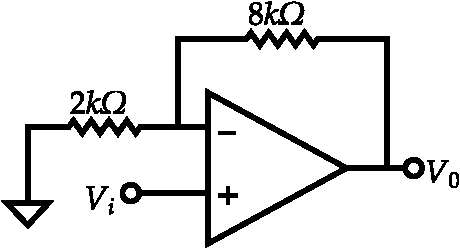
\includegraphics[height=2.8cm,width=5cm]{CE-2}
	\end{figure}
	 \begin{tasks}(4)
		\task[\textbf{a.}]20
		\task[\textbf{b.}]$4.5$
		\task[\textbf{c.}]4
		\task[\textbf{d.}] 5
	\end{tasks}
	\begin{answer}
		$$
		\begin{aligned}
		&\text { A closed loop gain, }\\
		A_{C L}&=\frac{V_{0}}{V_{i}}=\frac{A_{o d}}{1+\beta A_{o d}}, \beta=\frac{2 K}{8 K+2 K}=0.2, A_{C L}=\frac{45}{1+(45)(0.2)}=4.5
	\end{aligned}
	$$
	So the corrext answer is \textbf{Option (b)}
	\end{answer}
	\item  The circuit shown below uses only NAND gates. Find the final output. 
	\begin{figure}[H]
		\centering
		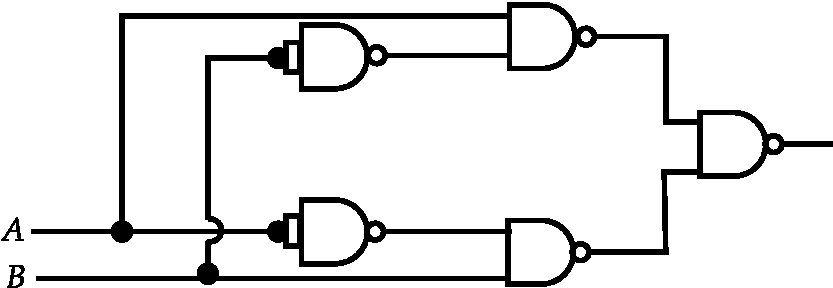
\includegraphics[height=2.8cm,width=8cm]{CE-3}
	\end{figure}
	 \begin{tasks}(4)
		\task[\textbf{a.}]A XOR B
		\task[\textbf{b.}]$\mathrm{AOR} \mathrm{B}$
		\task[\textbf{c.}]A AND B
		\task[\textbf{d.}] A NOR B
	\end{tasks}
	\begin{answer}$\left. \right. $\\
		\begin{figure}[H]
			\centering
			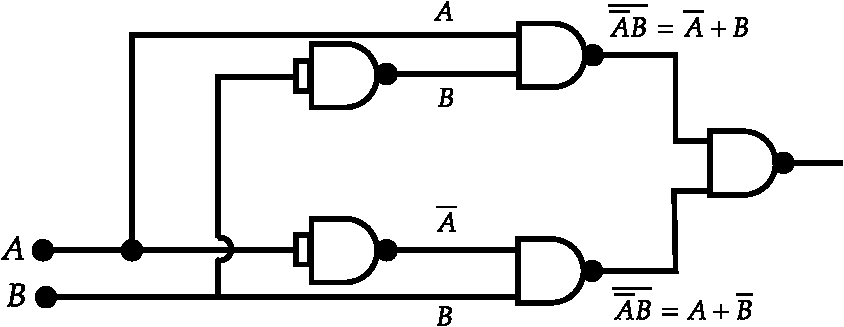
\includegraphics[height=3.3cm,width=8cm]{CE-4}
		\end{figure}
		$$
		\begin{aligned}
		\overline{(\bar{A}+B) \cdot(A+\bar{B})}=\overline{\bar{A}+B}+\overline{A+\bar{B}}=A \bar{B}+\bar{A} B=A X O R B
	\end{aligned}
	$$
		So the corrext answer is \textbf{Option (a)}
	\end{answer}
	\item In a digital circuit for three input signals $(A, B$ and $C)$ the final output $(Y)$ should be such that for inputs\\\\
	\begin{tabular}{lll}
		$\mathrm{A}$ & $\mathrm{B}$ & $\mathrm{C}$ \\
		\hline 0 & 0 & 0 \\
		0 & 0 & 1 \\
		0 & 1 & 0 \\
		\hline
	\end{tabular}\\\\
	the output (Y) should be low and for all other cases it should be high. Which of the following digital circuits will give such output ?
	 \begin{tasks}(2)
		\task[\textbf{a.}]\begin{figure}[H]
			\centering
			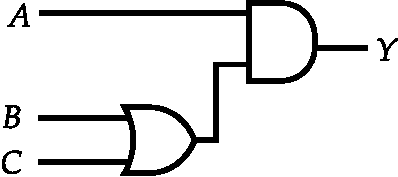
\includegraphics[height=1.7cm,width=4cm]{CE-5}
		\end{figure}
		\task[\textbf{b.}]\begin{figure}[H]
			\centering
			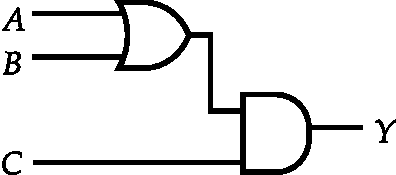
\includegraphics[height=1.7cm,width=4cm]{CE-6}
		\end{figure}
		\task[\textbf{c.}]\begin{figure}[H]
			\centering
			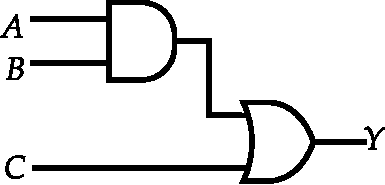
\includegraphics[height=1.7cm,width=4cm]{CE-7}
		\end{figure}
		\task[\textbf{d.}] \begin{figure}[H]
			\centering
			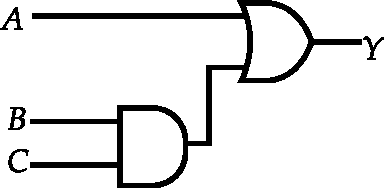
\includegraphics[height=1.7cm,width=4cm]{CE-8}
		\end{figure}
	\end{tasks}
	\begin{answer}
		$$
		\begin{aligned}
		\begin{array}{c|ccc}
		A & B & C & y \\
		\hline 0 & 0 & 0 & 0 \\
		0 & 0 & 1 & 0 \\
		0 & 1 & 0 & 0 \\
		1 & 0 & 0 & 1
		\end{array}
	\end{aligned}
	$$
	Only option (d) will give such output.\\
		So the corrext answer is \textbf{Option (d)}
	\end{answer}
	\item The mean kinetic energy of the conduction electrons in metals is ordinary much higher than $k T$ because
	 \begin{tasks}(1)
		\task[\textbf{a.}]Electrons have many more degrees of freedom than atoms do
		\task[\textbf{b.}] The electrons and the lattice are not in thermal equilibrium
		\task[\textbf{c.}]The electrons form a degenerate Fermi gas
		\task[\textbf{d.}] Electrons in metals are highly relativistic
	\end{tasks}
\begin{answer}
	The mean kinetic energy of the conduction electrons in metal is ordinary much higher than $\mathrm{kT}$ because the electrons form a degenerate fermi gas.\\
		So the corrext answer is \textbf{Option (c)}
\end{answer}
\item Which of the following statements concerning the electrical conductivities at room temperature of a pure copper sample and a pure silicon sample is NOT true ?
	[BHU 2012]
	 \begin{tasks}(1)
		\task[\textbf{a.}]If the temperature of the copper sample is increased, its conductivity will decrease
		\task[\textbf{b.}]If the temperature of the silicon sample is increased, its conductivity will increase
		\task[\textbf{c.}] The addition of an impurity in the copper sample always decreases its conductivity
		\task[\textbf{d.}]  The addition of an impurity in the silicon always decreases its conductivity
	\end{tasks}
\begin{answer}
		Out of above options, the option (d) "The addition of an impurity in the silicon always decreases its conductivity" is not type.\\
	So the corrext answer is \textbf{Option (d)}
\end{answer}
\item Indicate the statement about the semiconductors which is false ?
 \begin{tasks}(1)
	\task[\textbf{a.}] $n$-type semiconductors are obtained by doping phosphorus into silicon
	\task[\textbf{b.}]The conductivity of all semiconductors always increases with temperature
	\task[\textbf{c.}]$p$-type semiconductors are obtained by doping boron into silicon
	\task[\textbf{d.}] Intrinsic semiconductors are insulators at $T=0{ }^{\circ} \mathrm{K}$
\end{tasks}
\begin{answer}
Out of the above options, the option (b) the conductivity of all semiconductors always increases with temperature is false.\\
	So the corrext answer is \textbf{Option (b)}
\end{answer}
	\item Which of the following statements is true about the effective mass of electron in crystal?
	 \begin{tasks}(1)
		\task[\textbf{a.}]It is positive near the top of energy band 
		\task[\textbf{b.}]It is negative near the bottom of energy band
		\task[\textbf{c.}]It is constant through out the band
		\task[\textbf{d.}] It is negative near the top of energy band
	\end{tasks}
	\begin{answer}
	Out of the above options, "It is negative near the top of energy band"' is correct.
	So the corrext answer is \textbf{Option (d)}
	\end{answer}
\item Electrical conductivity of insulators is in the range:
	 \begin{tasks}(2)
		\task[\textbf{a.}]$10^{-10}(\Omega-\mathrm{mm})^{-1}$
		\task[\textbf{b.}]$10^{-10}(\Omega-\mathrm{cm})^{-1}$
		\task[\textbf{c.}] $10^{-10}(\Omega-\mathrm{m})^{-1}$
		\task[\textbf{d.}] $10^{-8}(\Omega-\mathrm{m})^{-1}$
	\end{tasks}
	\begin{answer}
	Electrical conductivity of intensity is in the range $10^{-8}(\Omega-\mathrm{m})^{-1}$. \\
	So the corrext answer is \textbf{Option (d)}
	\end{answer}
	\item Energy band gap size for semiconductors is in the ranges
	 \begin{tasks}(2)
		\task[\textbf{a.}]$1-2 \mathrm{eV}$
		\task[\textbf{b.}]$2-3 \mathrm{eV}$
		\task[\textbf{c.}]$3-4 \mathrm{eV}$
		\task[\textbf{d.}]  greater than $4 \mathrm{eV}$
	\end{tasks}
	\begin{answer}
	Energy band gap size for semiconductors is in the ranges $1-2 \mathrm{eV}$. \\
	So the corrext answer is \textbf{Option (a)}
	\end{answer}
	\item Fermi energy level for intrinsic semiconductors lies :
	 \begin{tasks}(2)
		\task[\textbf{a.}]At the middle of the band gap
		\task[\textbf{b.}]Close to the conduction band
		\task[\textbf{c.}]Close to valence band
		\task[\textbf{d.}] Inside valence band
	\end{tasks}
	\begin{answer}
		Fermi-level for intrinsic semiconductors lies at the middle of the band gap. \\
		So the corrext answer is \textbf{Option (a)}
	\end{answer}
	\item Indicate the false statement about the semiconductors
	 \begin{tasks}(1)
		\task[\textbf{a.}]All intrinsic semiconductors are insulators at $\mathrm{T}=0^{\circ} \mathrm{K}$
		\task[\textbf{b.}]At very high temperature all semiconductors become intrinsic semiconductors
		\task[\textbf{c.}] The conductivity of all semiconductors always increases with temperature
		\task[\textbf{d.}] N-type semiconductors are obtained by doping phosphorus into silicon
	\end{tasks}
	\begin{answer}
			Out of the given options, the option (c) the conductivity of all semiconductors always increases with temperature.\\
		So the corrext answer is \textbf{Option (c)}
	\end{answer}
\item The reverse saturation current in germanium $p-n$ diode is of the order of
	 \begin{tasks}(4)
		\task[\textbf{a.}]$n \mathrm{~A}$
		\task[\textbf{b.}]$\mu \mathrm{A}$
		\task[\textbf{c.}] $\mathrm{mA}$
		\task[\textbf{d.}] ampere
	\end{tasks}
	\begin{answer}
	The reverse saturation current in germanium $p-n$ junction diode is of the order of microampere ( $\mu \mathrm{A})$\\
		So the corrext answer is \textbf{Option (a)}
	\end{answer}
\item The Fermi level in an $n$-type semiconductor at $0{ }^{\circ} \mathrm{K}$
 \begin{tasks}(1)
	\task[\textbf{a.}]Lies below the donor level
	\task[\textbf{b.}]Lies in the conduction band
	\task[\textbf{c.}]Lies half-way between the conduction band and donor level
	\task[\textbf{d.}] Coincides with the intrinsic Fermi level
\end{tasks}
\begin{answer}
	The Fermilevel in an $n$-type semiconductor at $0{ }^{\circ} \mathrm{K}$ lies half-way between the conduction band and donor level.\\
	So the corrext answer is \textbf{Option (c)}
\end{answer}
\item If the Fermi energy of a metal at $0{ }^{\circ} \mathrm{K}, 10 \mathrm{eV}$, the mean energy of the electrons in the metal at $0{ }^{\circ} \mathrm{K}$ is
 \begin{tasks}(4)
	\task[\textbf{a.}]$6 \mathrm{eV}$
	\task[\textbf{b.}] $5 \mathrm{eV}$
	\task[\textbf{c.}]$1.5 \mathrm{eV}$
	\task[\textbf{d.}]  $2 \mathrm{eV}$
\end{tasks}
\begin{answer}
	$$
	\begin{aligned}
		&\text { The average energy of electrons in the metal at } 0{ }^{\circ} \mathrm{K} \text {, }\\
		\vec{E}&=\frac{3}{5} E_{f}=\frac{3}{5} \times 10 \mathrm{eV}=6 \mathrm{eV}
\end{aligned}
$$
	So the corrext answer is \textbf{Option (a)}
\end{answer}





\end{enumerate}